\documentclass{article}
\usepackage{url}
\usepackage{amsmath}
\usepackage{graphicx}
\usepackage[linesnumbered,lined,boxed,commentsnumbered]{algorithm2e}
\title{Bootstrapping phylogenies with allele frequencies for few hyperpolymorphic loci}

\begin{document}
\section{Introduction}

\begin{figure}
    \centering
    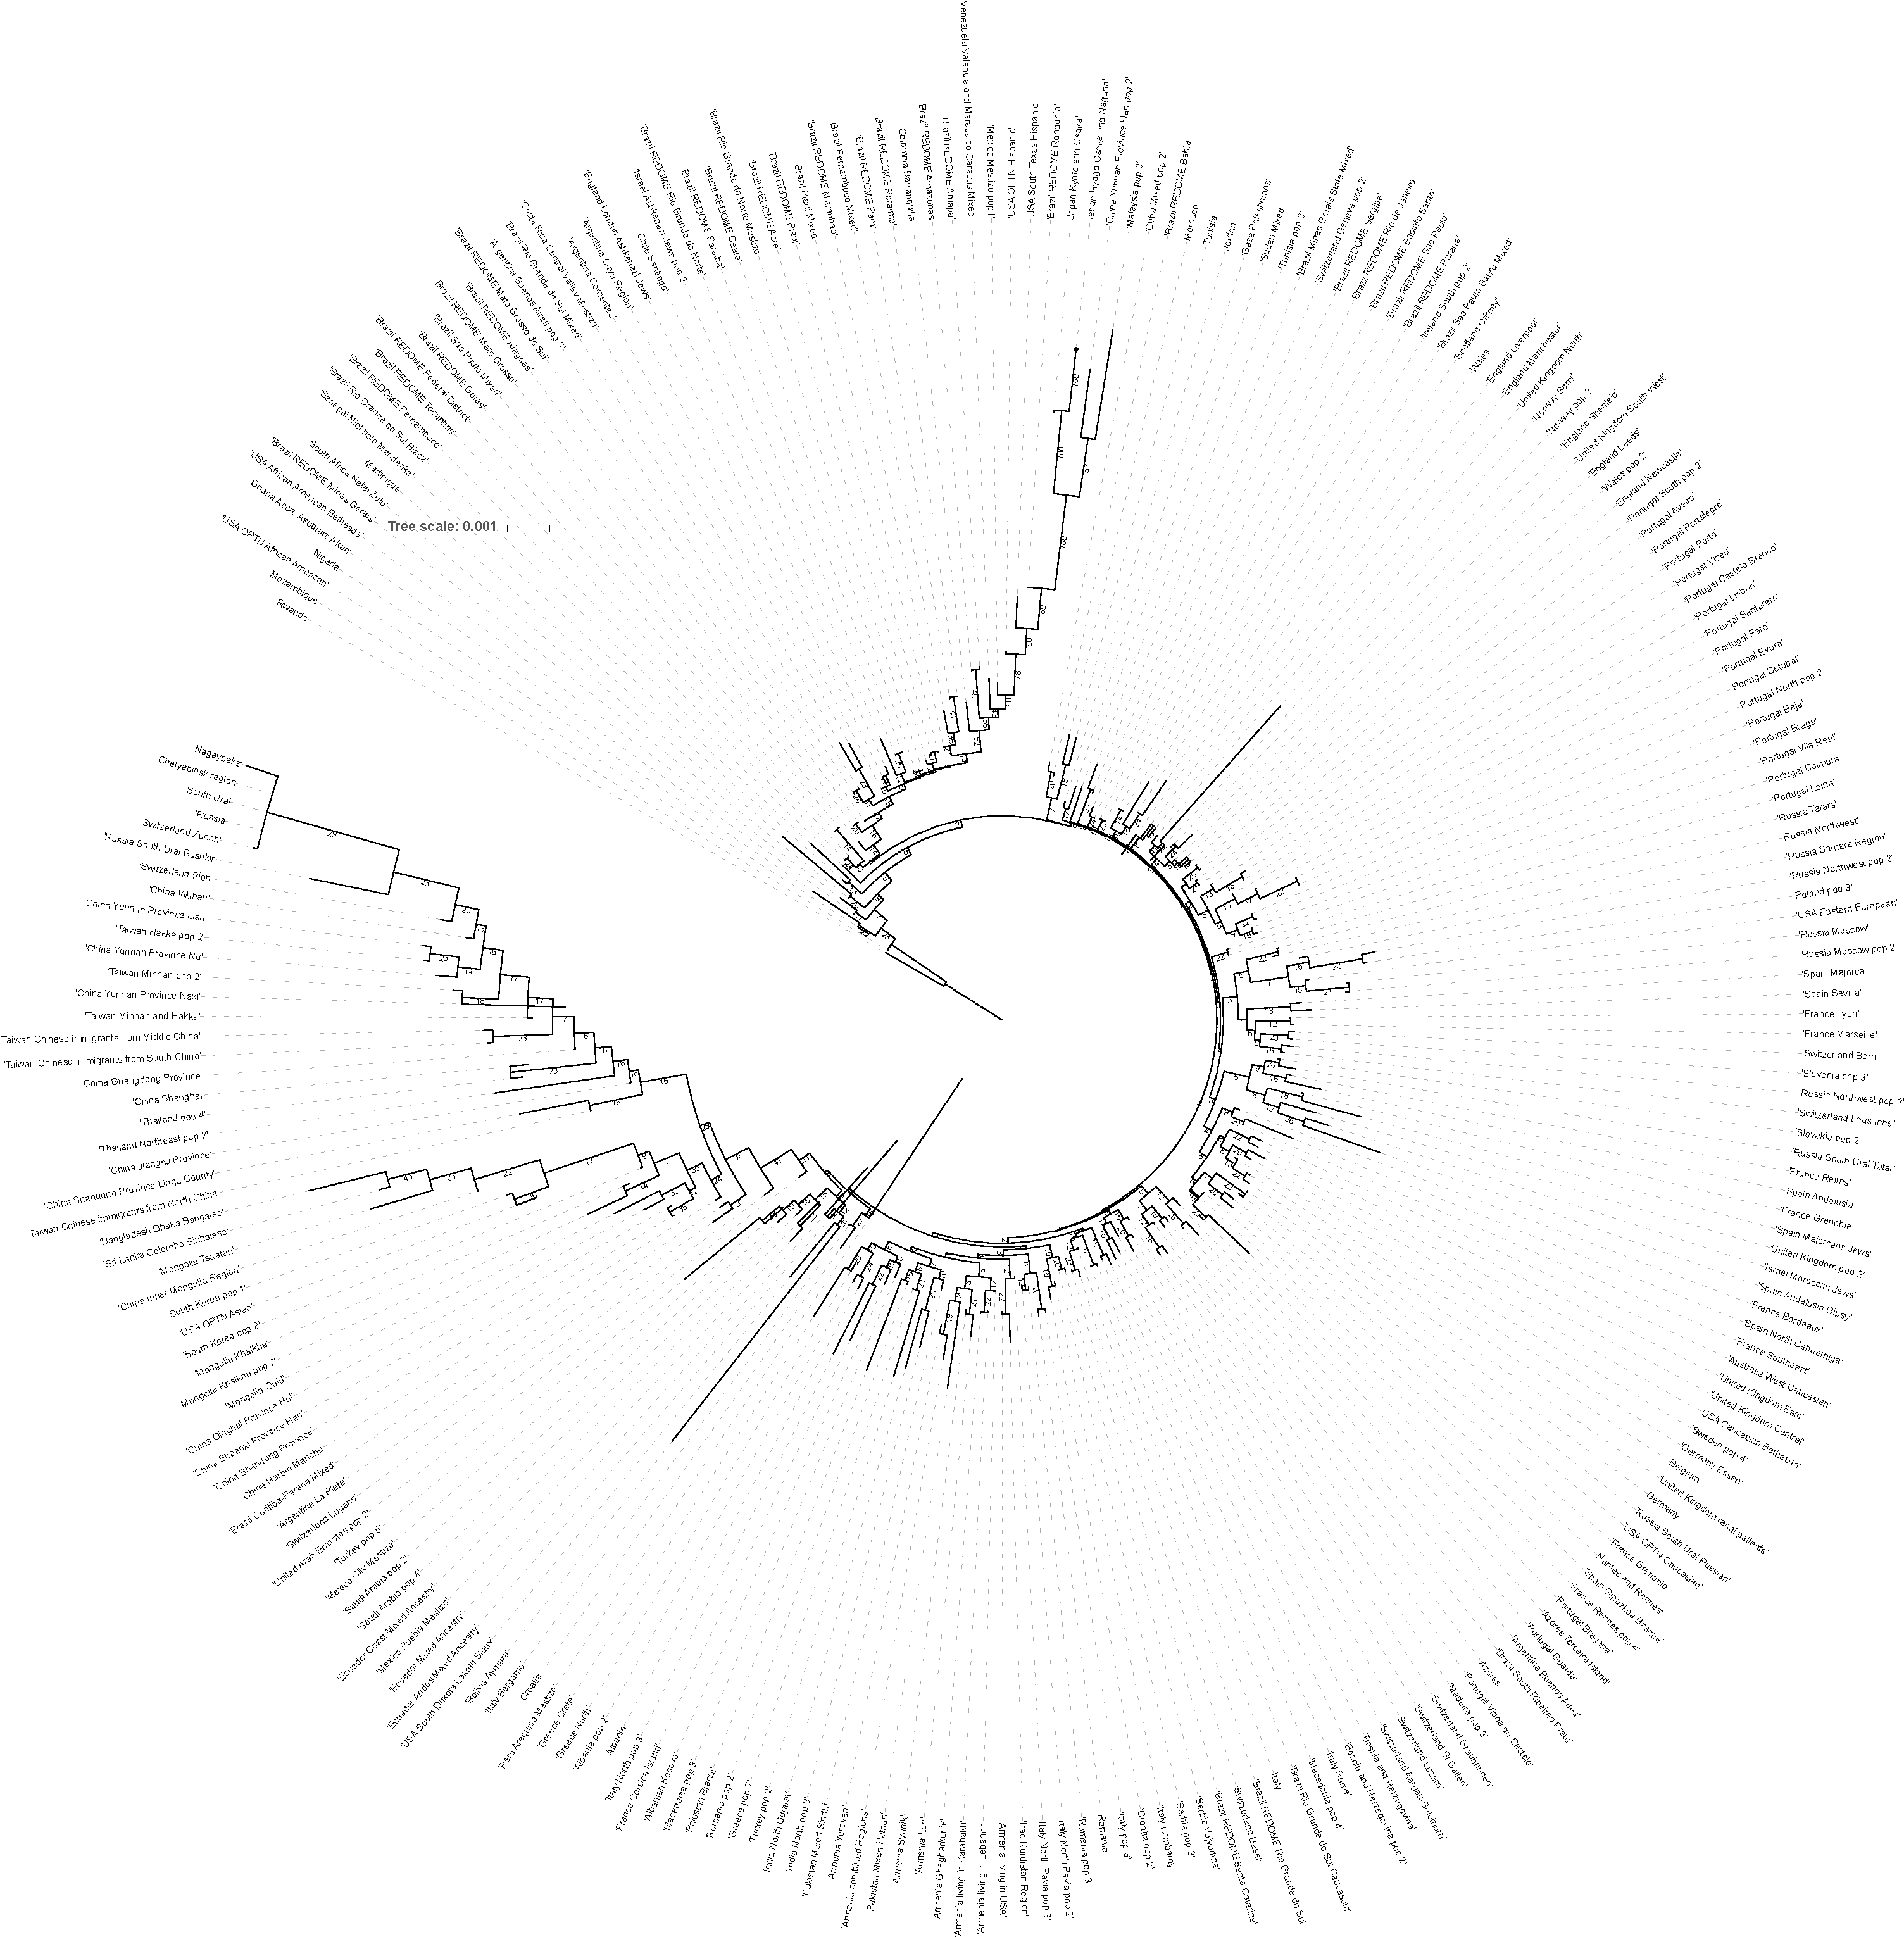
\includegraphics[width=\textwidth]{Figures/maj_AB_nj_246_99.pdf}
    \label{treeAB}
\end{figure}

%From Yurek's email, not sure whether to keep it, if so, back up by citations
There is a historic basis for using HLA gene frequencies in population studies. Mainly, there are six highly polymorphic
loci to choose between that have different frequencies between individuals and different populations. Class II genes
appear to be older than the class I genes[citation needed]. Although there is some trans-species HLA gene flow between human and apes,
trans speciation is relatively minor and loci dependent. Thus, most human HLA alleles, although old, have probably
evolved by genetic drift, selection and mutation with gene flow and admixture contributing to the polymorphisms in the
MHC region since the split between apes and humans.


It is also claimed that HLA is under selection, which raise concerns %% TODO: elaborate
%argue that it is still feasible for our purposes!


Nonetheless, hyperpolymorphic genes such as HLA class I and II are frequently used in anthropological and population genetic studies.
HLA typing has its roots in serology and thus experimentally, large body of data is available.
%Yurek "phylogenies from few albeit polymorphic loci"
Because of their enormous polymorphism and differences between individuals and populations, the phylogenies of HLA genes
are in theory highly informative for population genetics and anthropology. From an information theoretic perspective
they are a promising research target, as the amount of all possible outcomes
However, current methods are based on allele frequencies alone and do not leverage the information theoretic richness during bootstrapping:
Bootstrapping is based on random sampling with replacement from the original input. To the best of our knowledge,
all phylogenetic toolkits that are capable of dealing with allele frequencies sample gene-wise.
I.e, either a gene is sampled and all its allele frequencies (in the case of HLA genes, this can be as high as ...)
are considered or the gene is discarded in a bootstrap and then none of its allele frequences are taken into
account. This all-or-nothing approach works well when many loci are considered (e.g. microsatellites)
but for few genes, it leads to a very coarse grained information entropy resolution.

%The entirety of variation on those genes
Rich databases describing
Therein, populations are described in terms of allele frequencies (see allelefrequenciens.net paper)
Unfortunately, the low number of genes as biomarkers in combination with phylogenetic tools that expect high numbers of
loci for bootstrapping have led to numerous works with incorrect bootstrapping.
They providing false confidence into produced phylogenetic trees. The ramifications of such practices have caused
severe controversies:
In 2002, Piazza, Risch and Cavalli-Sforza have already criticized the works of Hajjej/Arnaiz-Villena and noted that
phylogenetic analysis  "Using results from the analysis of a single marker, particularly one likely to
have undergone selection, for the purpose of reconstructing genealogies is unreliable and unacceptable
practice in population genetics"

Nonetheless, a large number of HLA-based phylogeny reconstruction publications have since been  published based on one
or very few marker genes \cite{}.
It is worth noting that HLA genes are hyperpolymorphic, and as such many columns in respective MSAs would carry
information entropy for population genetics studies. Most tree reconstruction methods assume locus independence
(\cite{Efron1996Nov}), which yet requires a rigorous examination. The problem is not necessarily the low number of
gene markers as long as they are hyperpolymorphic (i.e., respectively contain multiple polymorphic nucleotide loci)
and representative enough for a species' genome or population's genepool.

Most phylogenetic tools used for tree reconstruction from allele frequencies are not suitable for low numbers of marker
genes (Phylip, DISPAN, check GenPop), since they perform bootstrapping with loci (i.e., here: genes) as units.
If only allele frequencies from a single gene are used, conventional bootstrapping performs resampling with replacement,
draws repeatedly from only a single locus. Trivially, this single locus is in agreement with itself, and the tools
report 100\% branch support for all clades in the tree.
False confidence
Respected journals have failed to critically review this misuse of bootsrapping \cite{Villena2017Jan,Hajjej2018Mar}.
For two genes A and B, resampling leads the combinations AA (25\%), AB (50\%) and BB (25\%). If both A and B agree on the branch split
100\% branch split support will be reported by teh software. branch split is
supported by both A and B, 100\
as for example is the case in \cite{Hajjej2018Mar}.


%of large data sets of population specific
We here propose a method that constructs population phylogenies for HLA allele frequencies in combination with well structured databases
with deep sequencing data for those genes.

Rich databases such as AlleleFrequencies.net help to obtain population specific descriptions in terms of allele
frequencies. Subsequently, mapping of alleles to probabilistic sequence representations enable
the expression of equivalent information as position specific weight matrices or classic multiple sequence alignments.
 This mapping is facilitated by comprehensive and wellstructured databases such as IMGT.
With the algorithmic transition of gene markers to nucleotide markers
the number of informative loci increases by orders of magnitude.
This in turn consitutes an important prerequisite for the application of classic consensus tree construction and
bootstrapping, as resampling from this much larger pool of loci is
statistically more meaningful.

%%
%% Author: ahenschel
%% 4/21/19
%%

%HLA-A Genomic Sequence Alignments
%IPD-IMGT/HLA Release: 3.31.0
%Sequences Aligned: 2018 January 19
%Steven GE Marsh, Anthony Nolan Research Institute.
%Please see http://hla.alleles.org/terms.html for terms of use.


\section{Methods}

We download complete multiple sequence alignments from IPD-IMGT/HLA release 3.31.0. %TODO describe download source/date
For all genes for which multiple sequence alignments are available, we parse the respective alignment file
as obtained from IMGT (ref). The Python script is available at the github repository
\url{https://github.com/HenschelLab/FreqRT}.


%As our current focus is on two-digit resolution
%(driven by the majority of population data in AlleleFrequencies.net), we extract information of polymorphic sites from IMGT's
%gene files
As we are aiming to capture the entirety of genetic variability associated with HLA genes/alleles, we
parse for each HLA gene $g$ its respective multiple sequence alignment into Position Weight Matrices
(PWM, \cite{stormo1982use}) by associating each sequence to the allele identified by the first two digits of the
sequence identifier. This yields one PWM for each allele $A$, which we denote $W_{A}$.

In turn, given $m$ selected genes, we describe a population $P$ as a set of $m$ PWMs $W^P_g$, which are the weighted sum of the respective allele PWMs
\begin{equation}
    W^P_g = \sum_{A\in\mathcal{A}(g)} f_A^P W_{A}
\end{equation}
where $f_A^P$ is the frequency of allele $A$ in population $P$ and $\mathcal{A}(g)$ denotes the set of
all alleles for $g$.

\begin{algorithm}
    \SetKwInOut{Input}{input}\SetKwInOut{Output}{output}
    \Input{Selected genes: $G_1\ldots G_m$, Allele frequencies $f_{A_j}^{P_i}$ for $n$ populations $P_1\ldots P_n$ }
    \Output{Phylogenetic tree $T$ for $P_1\ldots P_n$ with bootstrap values}
    Preprocessing: Download MSAs from IMGT, $\forall j$ generate $W_{A_j}$

    \For{$P \in P_1\ldots P_n$} {
        \For{$g \in G_1\ldots G_m$} {
            $W^{P}_g \leftarrow \sum_{A\in\mathcal{A}(g)} f_A^{P} W_{A}$
        }
    }
    \For{$\mathit{bootstrap} \leftarrow 1$ \KwTo $1000$} {
        \For{g $\in G_1\ldots G_m$} {
           $\overline{W^P_g}$ = RandomResamplingColumns($W^P_g$) such that $|\overline{W^P_g}| = |W^P_{g}|$
        }
        Calculate distance Matrix DM, performing pairwise Nei distance calculations between populations

        \For{$P_i \in P_1\ldots P_n$} {
            \For{$P_j \in P_{i+1}\ldots P_n$} {
                $DM_{ij}$ = Nei($\overline{W^{P_i}_g}$ , $\overline{W^{P_j}_g}$ )
            }
        }

        $T_{\mathit{bootstrap}}$ = TreeConstruction($DM$)
    }
    Combine bootstrap trees $T_{\mathit{bootstrap}}$ to majority tree $T$ with bootstrap values

\end{algorithm}


%From old HLA paper
%In addition to the locally collected HLA class I data, we acquire allele frequencies for HLA-A and HLA-B from
%AlleleFrequencies.net [1] using the web site's automated access method for a comprehensive list of population reference codes.
%We also considered HLA-C frequencies which however is only available for substantially fewer populations;
%moreover HLA-B and HLA-C are in linkage disequilibrium.
%We selected populations from continents neighboring the Middle East region if they passed the following quality control criteria:
%we rule out populations if allele frequencies were reported for different resolutions and yielded contradicting values,
%i.e, when subtype frequencies would not add up to the frequency of the corresponding supertype. Further we discard populations for which frequencies would not at least add up to 85% per locus. If frequencies would exceed 100% per locus (e.g., due to rounding errors), we normalize the frequencies such that their sum yields 100%.
%The final selection of populations was conducted manually, taking relevance, uniqueness and population size into account.
%The phylogenetic tree was calculated by first producing a distance matrix amongst for all selected populations using GENDIST from the PHYLIP package[2], which implements  Nei's standard genetic distance. Subsequently we calculate a Neighbor Joining tree, which is visualized in iToL [3].


\section{Conclusions}

The wrong practice of bootstrapping seems to be relatively common place in the HLA community.
We would hereby like to raise awareness during three time points of the publication cycle. First, software tools like
Phylip, DISPAN etc ought to generate warnings, when the number of provided loci is too low to subject allele frequencies to
bootstrapping. Secondly, naturally scientists creating phylogenies should know what they are doing. Finally, journals like
PLoS ONE need to improve review procedures for population phylogenys built with allele frequencies, in particular those with
just one or few loci.

\bibliography{ref}
\bibliographystyle{ieeetr}


\end{document}
